\begin{center}
            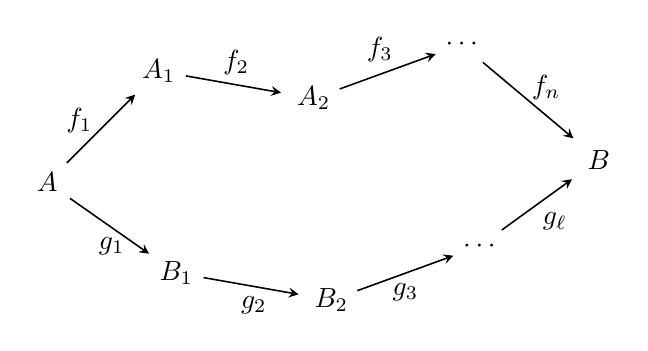
\begin{tikzpicture}[line width = 0.2mm, >=stealth, shorten >= 12pt, shorten <=10pt]
                \draw[->, Black] (0,0) coordinate (a)
                -- node[above, xshift = -0.3cm, yshift = -0.2cm] {$f_1$} ++(45:2) coordinate (b);
                \draw[->, Black,] (b)
                -- node[above] {$f_2$} ++(-10:2) coordinate (c);
                \draw[->, Black, shorten >= 10pt] (c)
                -- node[above, xshift = -0.1cm] {$f_3$} ++(20:2) coordinate (d);
                \draw[->, Black] (d)
                -- node[above, xshift = 0.2cm, yshift = -0.1cm] {$f_n$}++(-40:2.275) coordinate (e);
                \node[] at (a) {$A$};
                \node[] at (b) {$A_1$};
                \node[] at (c) {$A_2$};
                \node[] at (d) {$\cdots$}; 
                \node[] at (e) {$B$};
        
                \draw[->, Black] (0,0)
                -- node[below] {$g_1$}++(-35:2) coordinate (f);
                \draw[->, Black] (f)
                -- node[below] {$g_2$}++(-10:2) coordinate (g);
                \draw[->, Black, shorten >= 10pt] (g)
                -- node[below] {$g_3$}++(20:2) coordinate (h);
                \draw[->, Black] (h)
                -- node[below, xshift = 0.2cm] {$g_{\ell}$} (e);
                \node[] at (f) {$B_1$};
                \node[] at (g) {$B_2$};
                \node[] at (h) {$\cdots$};
            \end{tikzpicture}
        \end{center}